\section{Introduction}

\begin{figure*}[t]
    \centering
    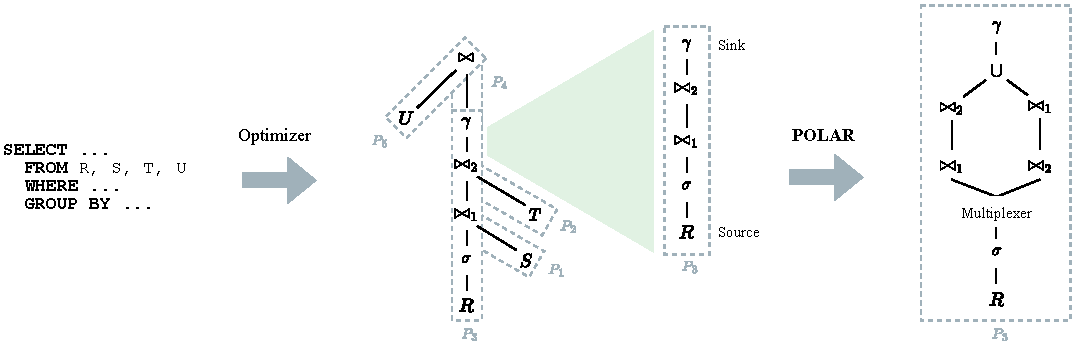
\includegraphics[width=0.9\textwidth]{figures/polar_pipeline-4.pdf}
		\vspace{-0.5cm}
		\caption{POLAR pipeline compilation from input query via standard, pipelined plan to POLAR pipelines.}
    \label{fig:pipeline_design}
		\vspace{-0.1cm}
\end{figure*}

% context
Cost-based query optimizations \cite{SelingerACLP79,moerkotte23} for selecting optimal join orders, join methods, and data access paths are crucial for the end-to-end performance of analytical queries. State-of-the-art exact join ordering algorithms such as DPsize~\cite{SelingerACLP79,HanKLLM08}, DPsub, DPcpp~\cite{MoerkotteN06}, and DPhyp~\cite{MoerkotteN08} rely on dynamic programming for efficient enumeration and are agnostic to used cost model and cardinality estimates. These algorithms yield optimal execution plans, but only under the assumption of precise cardinality estimates. 

\textbf{Cardinality Estimation Challenges:} Estimating precise cardinalities for intermediate results of complex queries remains a stubbornly difficult problem~\cite{LeisGMBK015}. Inaccuracies stem from multiple sources. First, most systems assume uniform distributions (no skew) and independence of predicates (no correlation) \cite{IlyasMHBA04}. These simplifying assumptions often cause under-estimation, which is problematic due to plan choices with poor asymptotic behavior~(\eg nested-loop joins), which perform poorly for larger intermediates \cite{IlyasMHBA04,LeisGMBK015}. Second, missing or too coarse-grained statistics (\eg histograms \cite{KanneM10} or sketches \cite{IzenovDRS21}) can cause deviations for clustered data. Third, user-defined functions and new environments (\eg cloud, federated, raw data) often do not allow obtaining statistics \cite{HueskePSRBKT12,JosifovskiSHL02,ReyFN23}. Fourth, complex queries with many operators are difficult to estimate because errors propagate exponentially \cite{IzenovDRS21,IoannidisC91,MoerkotteNS09}. Although recent work on ML-based estimators \cite{KipfKRLBK19,DuttWNKNC19,YangLKWDCAHKS19}, learning to distrust certain estimates \cite{MarcusNMZAKPT19}, and learning to rank plans \cite{BehrMK23} offer benefits, they do not solve all problems above.

\textbf{Adaptive Query Processing (AQP):} In the past two and a half decades, a spectrum of AQP techniques \cite{BabuB05,DeshpandeIR07,IvesDR07,DeshpandeHR06} has been devised to address the challenges of unknown and changing data characteristics. Many AQP techniques follow the classical MAPE control loop of monitoring, analyzing, planning, and executing \cite{IvesDR07,mape05,AboulnagaHLLMPR04}. Existing techniques include inter-query optimization with learned cardinalities for expressions \cite{BrunoC02,ChenR94,StillgerLMK01}, late binding with re-optimization at pipeline breakers \cite{DeshpandeHR06} or parameter binding \cite{BizarroBD09}, inter-operator re-optimization at checkpoint operators \cite{KabraD98}, progressive and pro-active re-optimization with validity ranges of cardinalities \cite{MarklRSLP04,BabuBD05}, intra-operator adaptivity with union stitch-up plans \cite{IvesHW04}, intra-query adaptivity via reinforcement learning in SkinnerDB \cite{TrummerWMMJA19,TrummerWWMMJAR21,WeiT22}, as well as tuple routing policies in Eddies \cite{HellersteinA00,Arpaci-Dusseau03,Deshpande04,BizarroBDW05}. Many of these strategies require both optimizer and runtime extensions for effective and efficient adaptivity.

\textbf{Robust Query Processing:} An alternative mitigation strategy for poor cardinality estimates is robust query optimization \cite{Haritsa20}. The influential Picasso project \cite{Haritsa10} on plan diagrams \cite{ReddyH05} revealed that state-of-the-art commercial DBMS compile many very specialized plans that are only optimal in a small subspace of actual cardinalities. Since these cardinalities are difficult to estimate, robust query processing seeks to find a small number of plans that cover the entire cardinality space, with each plan covering a broad range of cardinalities \cite{DDH07,DDH08}. Despite a sequence of valuable improvements \cite{DDH08,AbhiramaBDSH10,GraefeGKP12,DuttH14} (including so-called plan bouquets \cite{DuttH14}), many of these strategies are offline approaches and a recent PVLDB tutorial \cite{Haritsa20} concluded that robust query processing is largely intractable. 

\textbf{POLAR Overview:} Although AQP comprises many valuable ideas, only very few are implemented by data(base) systems in practice. We attribute this largely to the induced complexity of intertwining planning and execution, difficulties in testing and debugging, and potential performance regressions due to overheads of adaptivity. Inspired by tuple-routing and self-scheduling (queue-based) systems, we introduce POLAR as a novel adaptive processing approach of join pipelines. We enhance left-deep join pipelines with alternative join orders during planning, perform regret-bounded tuple routing for exploration, and process most data through \emph{plans of least resistance} (i.e., plans with few intermediates). In contrast to tuple routing in Eddies and SkinnerDB, POLAR is non-invasive to the optimizer and runtime, has low and bounded overhead, and does not require state management (e.g., partially-built hash tables).

\textbf{Contributions:} Our primary contribution is the concept of plans of least resistance (POLAR) as a new AQP technique designed for simple system integration and low overhead. We use our prototypical implementation in DuckDB~\cite{RaasveldtM19} to extensively evaluate POLAR’s performance. Our detailed contributions are:
\begin{itemize}
    \item \emph{Pipeline Design:} We introduce the pipeline design, join order selection strategies, and pipeline processing, including performance tracking and parallel execution (Section~\ref{pipeline-design}).
    \item \emph{Routing Strategies:} We propose an extensible multiplexer operator and four routing strategies, as well as describe their trade-offs and runtime characteristics (Section~\ref{sec:routing_strategies}).
    \item \emph{Experiments:} Using a variety of benchmarks, we study the performance characteristics of POLAR in DuckDB. We evaluate different join order selection and routing strategies and compare with database and AQP systems (Section~\ref{experiments}).
\end{itemize}
